% \documentclass{report}

% \usepackage[ english, greek]{babel}
% \usepackage[utf8]{inputenc}
% \usepackage[LGR, T1]{fontenc}

% % % 

% \newcommand{\tl}{\textlatin}
% \newcommand{\en}{\selectlanguage{english}}
% \newcommand{\gr}{\selectlanguage{greek}}

% \usepackage{hyperref}  % package for linking figures etc
% \usepackage{enumitem}  % package for description with bullets
% \usepackage{graphicx}  % package for importing images
% \usepackage{mathtools} % package for math equation
% \usepackage{mathrsfs}  % package for math font
% \usepackage{indentfirst} % package for getting ident after section or paragraph
% \usepackage{subcaption} % package for subfigures
% \usepackage[export]{adjustbox}
% \usepackage{longtable} % package for multi pages tables
% \usepackage{multirow}  % package for tables, multirow
% \usepackage{amssymb}
% \usepackage{esvect}
% \usepackage[
% backend=bibtex,
% citestyle=authoryear,
% % citestyle=authoryear-comp,
% % citestyle=authoryear-ibid,
% bibstyle=numeric,
% sorting=ynt,
% % style=numeric,
% % style=alphabetic ,
% ]{biblatex}
% \addbibresource{References}

% \graphicspath{ {./theory/figures/} }       % path for images

% \begin{document}
\gr 
 
\chapter{\gr Αλγόριθμος σύνδεσης των \en action tubes\gr}

Στο προηγούμενο κεφάλαιο περιγράψαμε μεθόδους για την παραγωγή υποψήφιων \en ToIs\gr, δεδομένου ενός μικρού τμήματος βίντεο που διαρκεί 8 ή 16 καρέ. Ωστόσο, τα πραγματικά βίντεο και πραγματικές ανθρώπινες ενέργειες, σε εξωτερικές συνθήκες, διαρκούν πάνω από 16 καρέ τις περισσότερες φορές. Τα τρέχοντα δίκτυα δεν είναι σε θέση να επεξεργαστούν ένα ολόκληρο βίντεο με την μία, προκειμένου να προτείνει υποψήφια \en ToIs\gr,
λόγω προβλημάτων μνήμης και υπολογιστικής ενέργειας.
Πολλές προσεγγίσεις για εντοπισμό δράσης λύνουν αυτό το πρόβλημα, δεδομένου ενός βίντεο, είτε
προτείνουν υποψήφιες περιοχές σε επίπεδο καρέ και, στη συνέχεια, τις συνδέουν με σκοπό τη δημιουργία υποψήφιων \en action tubes\gr, είτε
το διαχωρίζουν σε τμήματα βίντεο, προτείνοντας ακολουθίες από δισδιάστα πλαίσια τα οποία στην συνέχεια συνδέουν για να δημιουργήσουν
\en action proposals\gr.
Και οι δύο προαναφερθείσες προσεγγίσεις καθιστούν την κατάλληλη επιλογή της μεθόδου σύνδεσης σημαντικό παράγοντα για την απόδοση του δικτύου.
Αυτό συμβαίνει επειδή, παρόλο που στο επίπεδο καρέ ή στο επίπεδο τμήματος βίντεο
οι προτάσεις μπορεί να είναι πολύ καλές, αν ο προτεινόμενος αλγόριθμος σύνδεσης δεν λειτουργεί καλά, οι τελικές προτάσεις \en action tubes \gr
δεν θα είναι αποτελεσματικές, οπότε το τελικό μοντέλο δεν θα
είναι σε θέση να επιτύχει υψηλή απόδοση ταξινόμησης.
Με άλλα λόγια, αν ο αλγόριθμος σύνδεσης δεν δημιουργεί προτάσεις δράσης με μεγάλο \en recall \gr και καλή απόδοση \en MABO\gr,
ο ταξινομητής του μοντέλου δεν θα είναι σε θέση να εκτελέσει την κατάλληλη ταξινόμηση, επειδή πιθανώς θα του έχουν δοθεί \en action tubes \gr χωρίς κανένα περιεχόμενο.
Σε αυτό το κεφάλαιο, παρουσιάζουμε 3 διαφορετικές προσεγγίσεις που χρησιμοποιούνται για τη σύνδεση των προτεινόμενων ToIs που παράγονται από το \en TPN \gr του προηγούμενου κεφαλαίου.

\section{Πρώτη προσέγγιση: συνδυασμός επικάλυψης και πιθανότητας δράσης}
Ο αλγόριθμος μας εμπνέεται από την προσέγγιση των \en\cite{DBLP:journals/corr/HouCS17}\gr, η οποία υπολογίζει όλες τις πιθανές ακολουθίες των \en ToIs\gr. Για να βρει τα  καλύτερα υποψηφία \en action tubes\gr,
χρησιμοποιεί μια βαθμολογία που μας λέει πόσο πιθανό μια ακολουθία του TOIs είναι να περιέχει μια ενέργεια. Αυτή η βαθμολογία είναι ένας συνδυασμός 2 μετρικών:
\begin{description}
\item[ Πιθανότητα δράσης ή Δραστικότητα(\tl{Actioness}), ] που είναι η πιθανότητα ενός \en ToI \gr να περιέχει μια δράση. Αυτό το σκορ
  παράγεται από τα \en scoring layers \gr  του \en TPN\gr.
\item [Σκορ επικάλυψης μεταξύ των \en ToIs\gr, ] το οποίο είναι το \en IoU \gr των τελευταίων πλαισίων του πρώτου \en ToI \gr και των πρώτων πλαισίων του δεύτερου \en ToIs\gr.
\end{description}

Η παραπάνω πολιτική βαθμολόγησης μπορεί να περιγραφεί από τον ακόλουθο τύπο:

\[ S = \frac{1}{m} \sum_ {i=1}^{m} Actioness_i + \frac{1}{m-1} \sum_{j=1}^{m-1} Overlap_{j,j+1} \]

Για κάθε πιθανό συνδυασμό \en ToIs\gr, υπολογίζουμε το σκορ του όπως φαίνεται στην εικόνα \ref{fig:gr_connection_algo}.

\begin{figure}[h]
  \centering
  \en
  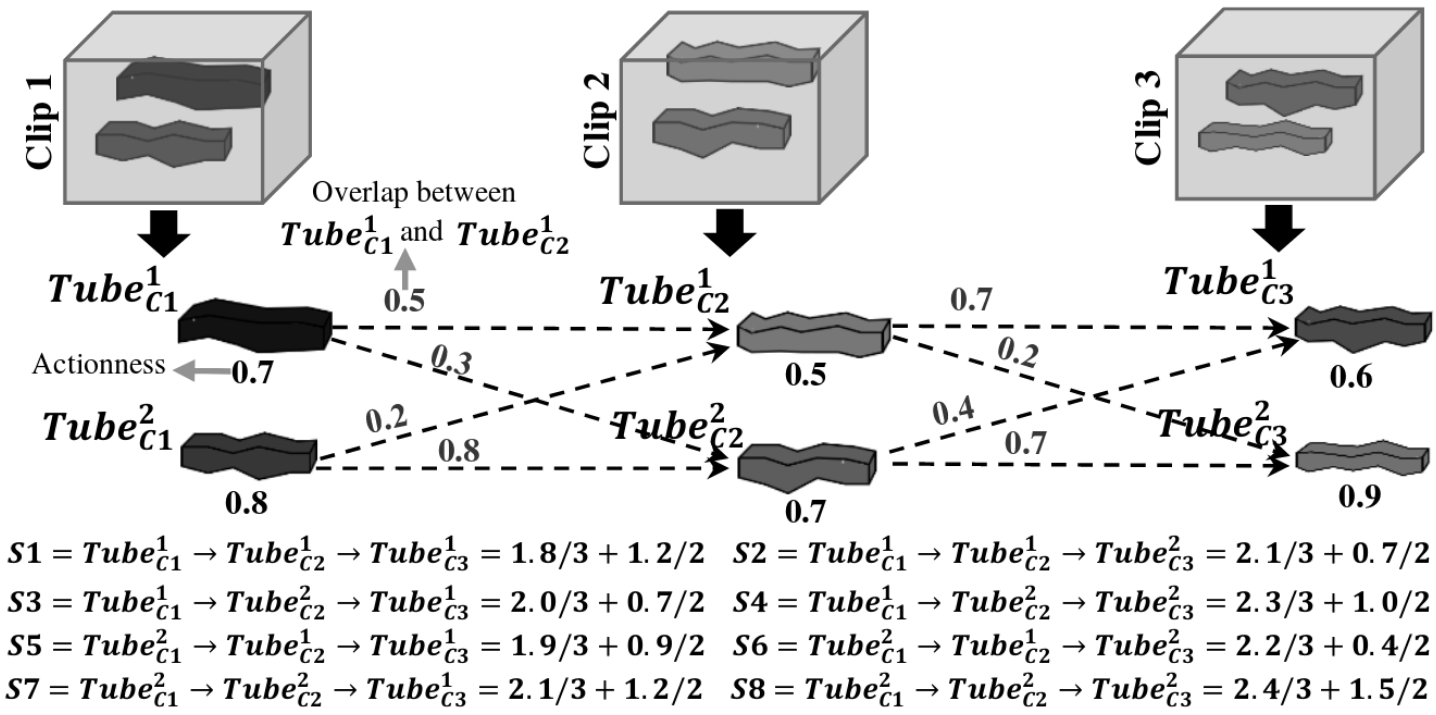
\includegraphics[scale=0.225]{connection_algo}
  \caption{An example of calculating connection score for 3 random TOIs taken from \cite{DBLP:journals/corr/HouCS17}}
  \label{fig:gr_connection_algo}
\end{figure}

Η παραπάνω προσέγγιση, όμως, χρειάζεται υπερβολικά πολύ μνήμη για την πραγματοποίηση όλων αυτών των υπολογισμών, έτσι
ένα πρόβλημα μνήμης εμφανίζεται. Ο λόγος είναι πως για κάθε νέο βίντεο κλιπ, εμείς προτείνουμε \en\textit{k ToIs} (\gr 16
κατά την διάρκεια της εκπαίδευσης και 150 κατά την διάρκεια του \en validation\gr.
Σαν αποτέλεσμα, για ένα μικρό βίντεο χωρισμένο σε \textbf{10 }μέρη, χρειάζεται να υπολογίσουμε τουλάχιστον
\textbf{$150^{10}$} σκορ κατά την διάρκεια της επικύρωσης. Αυτό οδηγεί το σύστημα μας να χρειάζεται υπερβολικά πολύ χρόνο
για να το πραγματοποιήσει.

Για να αντιμετωπίσουμε αυτό το πρόβλημα, δημιουργούμε έναν άπληστο αλγόριθμο για να βρούμε τα υποψήφια \en action tubes\gr.
Ο αλγόριθμος αυτός, για κάθε νέο τμήμα βίντεο, κρατά τα \en tubes \gr με βαθμολογία υψηλότερη από ένα κατώφλι και διαγράφει τα υπόλοιπα.
Έτσι, δεν χρειάζεται να υπολογίσουμε συνδυασμούς με πολύ χαμηλό σκορ. Γράψαμε κώδικα για τον υπολογισμό των βαθμολογιών των \en tubes \gr
στη γλώσσα \en CUDA\gr, η οποία έχει ως δυνατότητα την παράλληλη επεξεργασία του ίδιου κώδικα χρησιμοποιώντας διαφορετικά δεδομένα. Ο αλγόριθμος μας περιγράφεται παρακάτω:

\begin{enumerate}
\item Πρώτον, αρχικοποιούμε  κενές λίστες για τα τελικά \en tubes\gr,την διάρκεια τους, τις βαθμολογίες τους, τα ενεργά \en tubes\gr,
  τη διάρκειά τους, το άθροισμα των σκορ επικάλυψης  και δραστικότητας τους όταν:
  \begin{itemize}
  \item Η λίστα με τα τελικά \en tubes \gr περιέχει όλα τα \en tubes  \gr που είναι πιθανότερο να περιέχουν μια ενέργεια και η λίστα
    βαθμολογίας τους περιέχει τις αντίστοιχες βαθμολογίες τους. Αναφερόμαστε σε κάθε \en tube \gr από τον δείκτη του, ο οποίος
    σχετίζεται με ένα τένσορα, στον οποίο σώσαμε όλα τα \en ToIs \gr που προτείνονται από το \en TPN \gr για κάθε τμήμα βίντεο.
  \item Η λίστα ενεργών \en tubes \gr περιέχει όλα τα \en tubes \gr που θα συνδυαστούν με τα νέα \en  TOIs\gr.
    Η  λίστα άθροισης των επικαλυπτόμενων σκορ  και η λίστα άθροισης δραστικότητας περιέχουν τα αντίστοιχα αθροίσματα τους,
    προκειμένου να αποφεύγεται ο υπολογισμός τους για κάθε βρόχο. 
  \end{itemize}
Επίσης, ορίζουμε αρχικά  το όριο σύνδεσης ίσο με 0,5.
\item Για το πρώτο τμήμα βίντεο, προσθέτουμε όλα τα \en ToIs \gr τόσο στα ενεργά \en tubes \gr όσο και στα τελικά \en tubes\gr.
  Οι βαθμολογίες τους είναι μόνο η δική τους δραστικότητα επειδή δεν υπάρχουν \en tubes \gr για τον υπολογισμό της μεταξύ τους
  επικαλυπτόμενης βαθμολογίας. Έτσι, έτσι ορίζουμε το άθροισμα επικάλυψης ίσο με 0.
\item Για κάθε επόμενο βίντεο, μετά την λήψη των προτεινόμενων \en ToIs\gr, πρώτα υπολογίζουμε το σκορ επικάλυψης τους με κάθε
  ενεργό \en tube\gr. Μετά, αδειάζουμε την λίστα με τα ενεργά \en tubes\gr, με την διάρκεια τους, το άθροισμα επικάλυψης και το
  άθροισμα πιθανοτήτων δράσης. Για κάθε νέο \en tube \gr που έχει βαθμολογία υψηλότερη από το κατώφλι σύνδεσης
  προσθέτουμε τόσο στα τελικά \en action tubes \gr όσο και στα ενεργά, στις αντίστοιχες λίστες και αυξάνουμε τη διάρκειά τους.
\item Εάν ο αριθμός των ενεργών \en tubes \gr είναι μεγαλύτερος από ένα κατώτατο όριο, ορίζουμε το  όριο σύνδεσης ίσο με τη βαθμολογία του
  100ου καλύτερου \en tube\gr. Πέραν αυτού, ενημερώνουμε την τελική λίστα των \en tubes\gr, αφαιρώντας όλα τα \en tubes \gr
  που έχουν σκορ χαμηλότερο από το κατώφλι σύνδεσης.
\item Μετά από αυτό, προσθέτουμε στα ενεργά \en tubes\gr, τα προτεινόμενα \en ToIs \gr απ' το τρέχον τμήμα, μαζί με
  τα σκορ δραστικότητας στην λίστα με τα αθροίσματα δραστικότητας και μηδενικές τιμές στις αντίστοιχες θέσεις στην λίστα
  με τα σκορ επικάλυψης.
\item Επαναλαμβάνουμε τα προηγούμενα 3 βήματα μέχρι να μην έχει μείνει κανένα τμήμα βίντεο.
\item Τέλος, όπως αναφέραμε προηγουμένως, έχουμε μια λίστα που περιέχει τα ευρετήρια των αποθηκευμένων \en tubes\gr. Έτσι,
  τα τροποποιούμε  για να έχουμε  τα αντίστοιχα δισδιάστα πλαίσια. Ωστόσο, οι 2 διαδοχικά \en ToIs \gr δεν έχουν, πάντα,
  τα ίδια δισδιάστα πλαίσια  στα καρέ  που επικαλύπτονται. Για παράδειγμα, τα \en ToIs \gr από το πρώτο τμήμα βίντεο  ξεκινούν
  από το 1o καρέ έως το 16o καρέ. Εάν  έχουμε βήμα βίντεο ίσο με 8, αυτά τα \en ToIs \gr επικαλύπτονται χρονικά με  τα \en ToIs \gr
  από το δεύτερο τμήμα βίντεο στα καρέ 8-16. Σε αυτά τα πλαίσια, στο τελικό \en action tube\gr,
  επιλέγουμε την περιοχή που περιέχει και τα δύο πλαίσια οριοθέτησης που συμβολίζονται 
  ως $min(x_1,x'_1), min(y_1,y'_1), max(x_2,x'_2), max(y_2,y'_2))$ για τα δισδιάστατα πλαίσια $(x_1,y_1,x_2,y_2)$ και $(x_1,y_1,x_2,y_2)$.
\end{enumerate}

\subsection{\en JHMDB Dataset\gr}
Ξεκινώντας, θα ασχοληθούμε αρχικά μόνο με το \en JHMDB dataset  \gr προκειμένου να καθορίσουμε την πολιτική που ακολουθούμε για να υπολογίσουμε
το σκορ επικάλυψης. Kι αυτό γιατί τα βίντεο που περιέχει αυτό το σύνολο δεδομένων είναι πιο μικρά σε διάρκεια και λιγότερα στον αριθμό, οπότε
θα μπορέσουμε να βγάλουμε συμπεράσματα πιο γρήγορα απ' το να εξετάζαμε και τα δύο σύνολα δεδομένων ταυτόχρονα.

\paragraph{\gr Διάρκεια δείγματος ίση με  16 καρέ}
Ξεκινάμε ορίζοντας ως διάρκεια δείγματος ίση με 16 καρέ ανά βίντεο κλιπ. Αφού πραγματοποιήσαμε κάποια πρώτα πειράματα με βήμα βίντεο
ίσο με 8 και 12 καρέ, στα οποία δεν είχαμε καλές επιδόσεις σε \en recall\gr, αποφασίσαμε να εξετάσουμε την περίπτωση
του βήματος βίντεο ίσο με 14, 15 και 16 τα οποία παρουσιάζονται στον πίνακα \ref{table:gr_step14_16}. Για κάθε διαφορετικό βήμα βίντεο
έχουμε και διαφορετικές περιπτώσεις στις οποίες εξετάζουμε το σκορ επικάλυψης. Στις περιπτώσεις όπου έχουμε πάνω από 1 καρέ, λαμβάνουμε ως
σκορ επικάλυψης την μέση τιμή των σκορ επικάλυψης των αντίστοιχων καρέ. Στον \ref{table:gr_step14_16} αναφερόμαστε με πιο έντονο χρώμα στα καρέ, για τα οποία εξετάζουμε
την επικάλυψη τους.

\begin{center}
  \en
  \begin{longtable}{||c||c c c||}

  \hline
  \multirow{2}{5em}{combination} & {} &overlap thresh & {} \\
                                    &  0.5  &  0.4 &  0.3 \\         
  \hline  \hline
  0,1,...,13\textbf{\{14,15\}}                & {} & {} & {} \\
  \textbf{\{14,15\}},16,...,28,29                & 0.3731 & 0.5336 & 0.6493 \\
  \hline     \hline                          

  0,1,...,13,\textbf{\{14,\}}15,              & {} & {} & {} \\
  \textbf{\{14,\}}15,...,28,29                & 0.3694   & 0.5299 & 0.6455 \\
  \hline                          
  0,1,...,14,\textbf{\{15\}}                  & {} & {} & {} \\
  14,\textbf{\{15,\}}16,...,28,29             & 0.3731   & 0.5187 & 0.6381 \\
  \hline  \hline

  0,1,...,14,\textbf{\{15\}}                & {} & {} & {} \\
  \textbf{\{15\}},16,...,30                 & 0.3918 & 0.5187 & 0.6381 \\
  \hline     \hline                          
  0,1,...,14,\textbf{\{15\}}                & {} & {} & {} \\
  \textbf{\{16\}},17,...,31                 & 0.4067 & 0.7313 & 0.8731 \\
  \hline                          
  \caption{Recall results for steps = 14, 15 and 16}
  \label{table:gr_step14_16}
\end{longtable} 
\end{center}

Παρατηρούμε ότι έχουμε την καλύτερη επίδοση \en recall \gr για βήμα βίντεο ίσο με 16 καρέ όταν συγκρίνουμε
χωρικά την επικάλυψη του τελευταίου πλαισίου με την επικάλυψη του πρώτου.

\paragraph{\gr Διάρκεια δείγματος ίση με 8}

Θέλοντας να επιβεβαιώσουμε ότι έχουμε τα καλύτερα αποτελέσματα όταν έχουμε βήμα βίντεο ίσο με την διάρκεια του δείγματος,
εξετάσαμε και την περίπτωση να έχουμε διάρκεια δείγματος ίση με 8. Τα αποτελέσματα παρουσιάζονται στον πίνακα 
\ref{table:gr_step8_678 } και περιλαμβάνει τις περιπτώσεις όπου έχουμε βήμα βίντεο ίσο με 6, 7 και 8 καρέ.


\begin{center}
  \en
  \begin{longtable}{||c||c c c||}

  \hline
  \multirow{2}{5em}{combination} & {} &overlap thresh & {} \\
                                    &   0.5  &  0.4 &  0.3 \\         
  \hline  \hline
  0,1,2,3,4,5\textbf{\{6,7\}}           & {} & {} & {} \\
  \textbf{\{6,7\}},8,9,10,11,12,13      & 0.3134  & 0.7015 & 0.8619 \\
  \hline     \hline                          

  0,1,2,3,4,5,\textbf{\{6,\}}7          & {} & {} & {} \\
  \textbf{\{6,\}}7,8,9,10,11,12,13      & 0.3209  & 0.6679 & 0.847 \\
  \hline                          
  0,1,2,3,4,5,6,\textbf{\{7\}}          & {} & {} & {} \\
  6,\textbf{\{7\}}8,9,10,11,12,13       & 0.3172  & 0.6567 & 0.8507 \\
  \hline                          
  0,1,2,3,4,5,6\textbf{\{7\}}           & {} & {} & {} \\
  \textbf{\{7,\}}8,9,10,11,12,13,14     & 0.5597  & 0.7687 & 0.903 \\
  \hline                           
  0,1,2,3,4,5,6\textbf{\{7\}}           & {} & {} & {} \\
  \textbf{\{8\}}9,10,11,12,13,14,15     & 0.653	  & 0.8396 &0.9179  \\
  \hline                           
  \caption{Recall results for steps = 6, 7 and 8}
  \label{table:gr_step8_678 }
\end{longtable} 
\end{center}
Με βάση και τα αποτελέσματα του πίνακα \ref{table:gr_step8_678 } είναι πλέον ξεκάθαρο ότι πετυχαίνουμε καλύτερα αποτελέσματα όταν θέτουμε
το βήμα βίντεο ίσο με την διάρκεια του δείγματος και το σκορ επικάλυψης υπολογίζεται από το πλαίσιο του τελευταίου καρέ του πρώτου
\en ToI \gr με το πλαίσιο του πρώτο καρέ του δεύτερου \en ToI\gr.

\subsection {\en UCF Dataset\gr}
Σε προηγούμενα βήματα, προσπαθήσαμε να βρούμε την καλύτερη πολιτική επικάλυψης για τον αλγόριθμο μας στο σύνολο δεδομένων \en  JHMDB\gr.
Μετά από αυτό, είναι καιρός να εφαρμόσουμε τον αλγόριθμο μας στο σύνολο δεδομένων \en UCF \gr χρησιμοποιώντας την καλύτερη βαθμολογική
πολιτική επικάλυψης. Κάναμε κάποιες τροποποιήσεις στον κώδικα, για να χρησιμοποιούμε λιγότερη μνήμη, και μετακινήσαμε τα περισσότερα μέρη του κώδικα σε \en GPU\gr. Αυτό συνέβη με τη χρήση τένσορων αντί για  λίστες με βαθμολογίες ενώ oι περισσότερες πράξεις είναι, από τώρα και στο εξής,
πράξεις πινάκων. Πάνω σ' αυτό, το τελευταίο βήμα του αλγόριθμου, η οποία είναι η τροποποίηση από δείκτες σε πραγματικές ακολουθίες από
πλαίσια, είναι γραμμένο πλέον σε \en CUDA \gr κώδικα έτσι λαμβάνει χώρα και αυτή στη \en GPU\gr. Έτσι, τώρα μπορούμε να αυξήσουμε τον αριθμό των \en ToIs \gr που επιστρέφονται από το \en TPN\gr, τον μέγιστο αριθμό των ενεργών \en tubes \gr πριν από την ενημέρωση του ορίου και τον μέγιστο αριθμό τελικών
\en tubes\gr.  \par
Τα πρώτα πειράματα που διενεργήσαμε σχετίζονταν με τον αριθμό των τελικών σωλήνων, τα οποία το δίκτυο μας προτείνει, παράλληλα με τον αριθμό
των προτεινόμενων \en ToIs \gr  από  το \en TPN\gr. Πειραματιζόμαστε για υποθέσεις, στις οποίες το TPN προτείνει 30, 100 και 150 \en ToIs\gr, το τελικό δίκτυό μας προτείνει 500, 2000 και 4000 υποψήφια \en action tubes \gr για
διάρκεια δείγματος ίσο με 8 και 16 καρέ. Για διάρκεια δείγματος ίσο με 8 επιστρέφουμε 100 \en ToIs \gr επειδή, όταν
προσπαθήσαμε να επιστρέψουμε 150 \en ToIs\gr, λαμβάνουμε \en OutOfMemory \gr σφάλμα.
O πίνακας \ref{table:gr_ucf_recall} δείχνει τις αποδόσεις των χωροχρονικών \en recall \gr και \en MABO\gr,  αυτών των προσεγγίσεων.
O πίνακας \ref{table:gr_ucf_temp_recall} δείχνει την απόδοση των χρονικών \en recall \gr και \en MABO\gr.
Ενδιαφερόμαστε για τη χρονική απόδοση, επειδή το \en UCF  \gr αποτελείται από ατριμάριστα βίντεο, σε αντίθεση με το \en JHMDB \gr
που έχει μόνο τριμαρισμένα βίντεο. Έτσι, θέλουμε να γνωρίζουμε πόσο καλά το δίκτυό μας είναι σε θέση να προτείνει \en action tubes \gr που
επικαλύπτονται με τα πραγματικά \en action tubes \gr πάνω από ένα «μεγάλο» όριο.
Για χρονικό εντοπισμό, δεν χρησιμοποιούμε τα 0,5, 0,4 και 0,3 ως επικαλυπτόμενο όριο, αλλά αντ' αυτού, χρησιμοποιούμε 0,9, 0,8 και 0,7,
επειδή είναι πολύ σημαντικό το δίκτυό μας να είναι σε θέση να προτείνει \en action tubes \gr που
περιέχουν μια ενέργεια, τουλάχιστον από χρονικής απόψεως.
Για να υπολογίσουμε τη χρονική επικάλυψη, χρησιμοποιούμε το \en IoU \gr για μια μόνο διάσταση.

\begin{center}
\en
\begin{longtable}{||c | c | c ||c c c | c|}

  \hline
  \multirow{2}{*}{combination} & \multirow{2}{2.5em}{TPN tubes} & \multirow{2}{2.5em}{Final tubes} &  \multicolumn{3}{}{overlap thresh} & \multirow{2}{*}{MABO} \\
  {} & {} & {} &  0.5 &  0.4 & 0.3 & {}\\         
  \hline
  
  \multirow{6}{7em}{0,1,...,6,\textbf{\{7,\}}
  \textbf{\{8,\}}9,...,14,15 }  & \multirow{3}{*}{30} & 500   & 0.2829  & 0.4395 & 0.5817  & 0.3501 \\
  \cline{3-7}
  {} &  {}   & 2000   & 0.3567  & 0.4996 & 0.6289 & 0.3815\\
  \cline{3-7}
  {} &  {}   & 4000   & 0.3749  & 0.5316 & 0.6487 & 0.3934 \\
  \cline{2-7}
  {} &  \multirow{3}{*}{100}   & 500   & 0.2966  & 0.451 & 0.5947 & 0.356 \\
  \cline{3-7}
  {} &  {}   & 2000   & 0.3757  & 0.5163 & 0.6471 & 0.3902 \\
  \cline{3-7}
  {} &  {}   & 4000  & 0.3977  & 0.5506 & 0.6624 & 0.4029 \\
  \hline                                    
  \multirow{6}{7em}{0,1,...,14,\textbf{\{15,\}}
  \textbf{\{16,\}}17,18,...,23 }  & \multirow{3}{*}{30} & 500   & 0.362  & 0.5042 & 0.6243 & 0.3866 \\
  \cline{3-7}
  {} &  {}   & 2000   & 0.416  & 0.5468 & 0.6631 & 0.4108  \\
  \cline{3-7}
  {} &  {}   & 4000   & 0.4281  & 0.5589  & 0.6779 & 0.4182 \\
  \cline{2-7}
  {} &  \multirow{3}{*}{150}   & 500 & 0.3589  & 0.4981 & 0.6198 & 0.3845 \\
  \cline{3-7}
  {} &  {}   & 2000   & 0.4129  & 0.5392  & 0.6563 & 0.4085 \\
  \cline{3-7}
  {} &  {}   & 4000   & 0.4266  & 0.5521 & 0.6722 & 0.4162\\
  \hline                                    

  \caption{\en Recall results for UCF dataset}
  \label{table:gr_ucf_recall}
\end{longtable} 
\end{center}

\begin{center}
\en
\begin{longtable}{||c | c | c ||c c c| c|}

  \hline
  \multirow{2}{*}{combination} & \multirow{2}{2.5em}{TPN tubes} & \multirow{2}{2.5em}{Final tubes} &  {} &overlap thresh & {} & \multirow{2}{*}{MABO} \\
  {} & {} & {} &  0.9 &  0.8 & 0.7 & {}\\         
  \hline
  
  
  \multirow{6}{7em}{0,1,...,6,\textbf{\{7,\}}
  \textbf{\{8,\}}9,...,15 }  & \multirow{3}{*}{30} & 500   & 0.4464  & 0.581 & 0.6844  & 0.7787 \\
  \cline{3-7}
  {} &  {}   & 2000   & 0.635  & 0.7665 & 0.8403 & 0.8693 \\
  \cline{3-7}
  {} &  {}   & 4000   & 0.7034  & 0.8228 & 0.8875 & 0.8973 \\
  \cline{2-7}
  {} &  \multirow{3}{*}{100}   & 500   & 0.454 & 0.5924 & 0.692 & 0.783 \\
  \cline{3-7}
  {} &  {}   & 2000   & 0.651 & 0.7696 & 0.8441 &0.8734 \\
  \cline{3-7}
  {} &  {}   & 4000   & 0.7209 &0.8312 & 0.8913 & 0.9026 \\

  \hline                                    
  \multirow{6}{7em}{0,1,...,14,\textbf{\{15,\}}
  \textbf{\{16,\}}17,18,...,23 }  & \multirow{3}{*}{30} & 500   & 0.6844 &0.8327 & 0.9027 & 0.8992 \\
  \cline{3-7}
                                    {} &  {}   & 2000   & 0.7475 & 0.8684 & 0.9217 & 0.9175 \\
  \cline{3-7}
                                    {} &  {}   & 4000   & 0.7567  & 0.8745  & 0.9255 & 0.9211 \\
  \cline{2-7}
                                    {} &  \multirow{3}{*}{150}   & 500   & 0.7498 &0.8707 &0.9171 & 0.9125 \\
  \cline{3-7}
                                    {} &  {}   & 2000   & 0.8243 & 0.911 & 0.9392 & 0.9342\\
  \cline{3-7}
                                    {} &  {}   & 4000   &  0.8403  & 0.9179 & 0.9437 & 0.9389\\
  \hline                                    
  % \end{tabular}
  \caption{Temporal Recall results for UCF dataset}
  \label{table:gr_ucf_temp_recall}
% \end{table}
\end{longtable} 
\end{center}

Όπως φαίνεται και από τους πίνακες \ref{table:gr_ucf_recall} και \ref{table:gr_ucf_temp_recall}, για διάρκεια δείγματος ίση με 8 λαμβάνουμε
την καλύτερη επίδοση όταν επιστρέφει το \en TPN \gr 100 \en ToIs \gr και συνολικά το \en ActionNet  4000  action tubes\gr, ενώ
για διάρκεια δείγματος ίση με 16 καρέ όταν επιστρέφει το \en TPN, 30 ToIs \gr και το \en ActionNet  4000 action tubes.\gr \par

\subsubsection{Προτεινόμενη τροποποίηση του αλγορίθμου}

Στην προηγούμενη προσέγγιση, το κατώφλι σύνδεσης ανανεώνεται και αυξάνεται κάθε φορά ο αριθμός από «ενεργά» \en tubes \gr ξεπερνούν ένα
συγκεκριμένο αριθμό. Ωστόσο, παρατηρήσαμε ότι με αυτόν τον τρόπο το σύστημα μας αδυνατεί να προτείνει \en action tubes \gr τα οποία ξεκινούν
μετά από ορισμένα καρέ. Κι αυτό γιατί μέχρι τότε το κατώφλι σύνδεσης έχει αυξηθεί τόσο που δεν επιτρέπει να δημιουργηθούν νέα \en tubes \gr.
Για τον λόγο αυτό τροποποιήσαμε τον αλγόριθμο μας έτσι ώστε να μην ανανεώνεται το κατώφλι σύνδεσης. Παράλληλα, προσθέσαμε τον αλγόριθμο
\en NMS \gr προκειμένου να απορρίπτει \en action tubes \gr που επικαλύπτονται αρκετά με κάποια ήδη προτεινόμενα \en action tubes\gr.
Οι πίνακες \ref{table:gr_ucf_nms_noup_recall} και  \ref{table:gr_ucf_nms_noup_temp_recall} περιλαμβάνουν τα χωροχρονικά και χρονικά αποτελέσματα
για το \en recall \gr και το \en MABO\gr, ενώ πειραματιζόμαστε με κατώφλι σύνδεσης του \en NMS \gr ίσο με 0.7, 0.9 και χωρίς καθόλου \en
NMS\gr.

\begin{center}
  \en
  \setlength{\tabcolsep}{2pt}
\begin{longtable}{||c | c | c | c c c| c|}

  \hline
  \multirow{2}{*}{combination} & \multirow{2}{2.5em}{NMS thresh} & \multirow{2}{3.5em}{PreNMS tubes} &  {} &overlap thresh & {} & \multirow{2}{*}{MABO} \\
  {} & {} & {} &  0.5 &  0.4 & 0.3 & {}\\         
  \hline
  \multirow{3}{7em}{0,1,...,6,\textbf{\{7,\}}
  \textbf{\{8,\}}9,...,15 }   &   \multicolumn{2}{|c|}{-}     &  0.3779 & 0.5316 & 0.6471 & 0.393082961 \\
  \cline{2-7}
  {} & 0.7 &\multirow{2}{*}{20000}  & 0.3483  & 0.5194 & 0.6471 & 0.3783524086 \\
  \cline{2-2} \cline{4-7} 
  {} &  0.9   & {}   & 0.416 & 0.5605 & 0.6722 & 0.4074053106 \\
  \hline                                    
  \multirow{3}{7em}{0,1,...,14,\textbf{\{15,\}}
  \textbf{\{16,\}}17,...,23 }  &   \multicolumn{2}{|c|}{-} & 0.438 & 0.5635 & 0.6829 & 0.4231788 \\
  \cline{2-7}
  {} & 0.7 & \multirow{2}{*}{20000}   & 0.4525 & 0.5848 & 0.7034 & 0.429747438 \\
  \cline{2-2} \cline{4-7} 
  {} &  0.9   & {}   & 0.3802 & 0.5133 & 0.6068 & 0.3862278851848662 \\

  \hline                                    

  \caption{Spatiotemporal Recall results for UCF dataset}
  \label{table:gr_ucf_nms_noup_recall}
\end{longtable} 
\end{center}

\begin{center}
  \en
  \setlength{\tabcolsep}{2.2pt}
\begin{longtable}{||c | c | c | c c c| c|}

  \hline
  \multirow{2}{*}{combination} & \multirow{2}{2.5em}{NMS thresh} & \multirow{2}{3.5em}{PreNMS tubes} &  {} &overlap thresh & {} & \multirow{2}{*}{MABO} \\
  {} & {} & {} &  0.9 &  0.8 & 0.7 & {}\\         
  \hline

  \multirow{3}{7em}{0,1,...,6,\textbf{\{7,\}}
    \textbf{\{8,\}}9,...,15 }  &   -   & -    & 0.7087 & 0.8281 & 0.8913 & 0.899210587 \\
  \cline{2-7} 
  {} & 0.7 &\multirow{2}{*}{20000}  & 0.6586 & 0.854 & 0.9278 & 0.903373468 \\
  \cline{2-2} \cline{4-7} 
  {} &  0.9   & {}   &  0.8137 & 0.8973 & 0.9361 & 0.9333068498 \\
  \hline                                    
  \multirow{3}{7em}{0,1,...,14,\textbf{\{15,\}}
  \textbf{\{16,\}}17,...,23 }  &   \multicolumn{2}{|c|}{-} & 0.8327 & 0.9156 &0.9399 & 0.940143272 \\
  \cline{2-7}
  {} & 0.7 & \multirow{2}{*}{20000}& 0.8646 & 0.9369 & 0.9567 & 0.946701832 \\
  \cline{2-2} \cline{4-7} 
  {} &  0.9   & {}   & 0.6183 & 0.7696 & 0.8388 & 0.8628507037919737 \\
  \hline                                    

  \caption{Temporal Recall results for UCF dataset}
  \label{table:gr_ucf_nms_noup_temp_recall}
\end{longtable} 
\end{center}

Συγκρίνοντας τις επιδόσεις των \en recall \gr και \en MABO \gr που παρουσιάζονται στον Πίνακας \ref{table:gr_ucf_nms_noup_recall} μαζί με
αυτές του Πίνακα \ref{table:gr_ucf_recall}, συμπεραίνουμε πως για διάρκεια δείγματος ίση με 8, η νέα τροποποίηση οδηγεί σε χειρότερα αποτελέσματα
όταν το κατώφλι σύνδεσης είναι 0.7 αλλά καλύτερα για κατώφλι ίσο με 0.9 . Απ' την άλλη, για διάρκεια δείγματος ίση με 16, παρατηρούμε πως
έχουμε καλύτερα αποτελέσματα για κατώφλι σύνδεσης του \en NMS \gr αλγορίθμου ίσο με 0.7 .


\section{Δεύτερη προσέγγιση}
Όπως είδαμε και προηγουμένως, ο αλγόριθμος μας δεν έχει πάρα πολύ καλές \en recall \gr επιδόσεις. Έτσι, δημιουργήσαμε έναν άλλο αλγόριθμο
ο οποίος βασίζεται σε αυτόν που πρότειναν οι \en \cite{DBLP:journals/corr/abs-1903-00304}\gr.
Αυτός ο αλγόριθμος εισάγει δύο νέες μετρικές σύμφωνα με τους \en \cite{DBLP:journals/corr/abs-1903-00304}\gr.

% TODO add more description
\begin{description}
\item[ Πρόοδος  ] που περιγράφει την πιθανότητα μιας συγκεκριμένης δράσης να εκτελείται στο  \en ToI\gr.
 Προσθέτουμε αυτόν τον παράγοντα επειδή παρατηρήσαμε ότι η δραστικότητα είναι ανεκτική  σε ψευδώς θετικά. Η πρόοδος είναι
 ένα μηχανισμός επαναβαθμολόγησης για κάθε κατηγορία (όπως αναφέρονται οι  \cite{DBLP:journals/corr/abs-1903-00304})

\item [ Ρυθμός προόδου ] που ορίζεται ως η αναλογία προόδου κατά την οποία κάθε κατηγορία δράσης έχει πραγματοποιηθεί.
  
\end{description}

Έτσι, κάθε \en action tube \gr περιγράφεται ως ένα σύνολο \en TOIs \gr  
\[  T = {\{ {\bf t}_i^{(k)} | {\bf t}_i^{(k)} = ( t_i^{(k)}, s_i^{(k)}, r_i^{(k)} ) \}}_{i=1:n^{(k)},k=1:K} \]
όπου το $ t_i^{(k)} $ περιέχει τις χωροχρονικές πληροφορίες των \en TOI \gr, το   $ s_i^{(k)} $ το σκορ σιγουριάς του και
το $ r_i^{(k)} $ τον ρυθμό προόδου.

Σε αυτή την προσέγγιση, κάθε κλάση αντιμετωπίζεται ξεχωριστά, συνεπώς για την υπόλοιπη ενότητα
συζητάμε για την παραγωγή \en action tubes \gr μόνο για μία κλάση. Για τη σύνδεση 2 \en ToIs\gr, για
ένα βίντεο με \textit{N} τμήματα βίντεο , εφαρμόζονται τα ακόλουθα βήματα:

\begin{enumerate}
\item Για το πρώτο τμήμα βίντεο (\tl{k} = 1), προετοιμάζουμε έναν πίνακα με τα Μ καλύτερα \en ToIs\gr,  τα  οποία θα θεωρούνται
  ως ενεργά \en tubes\gr(AT).
Αντιστοιχα, προετοιμάζουμε έναν πίνακα με \textit{M} ρυθμούς προόδου και \textit{M} βαθμολογίες εμπιστοσύνης.
\item Για \en k = 2:N\gr, εκτελούμε τα βήματα (a') - (g'):
  \begin{enumerate}
  \item Υπολογίζουμε τις επικαλύψεις μεταξύ $ AT^{(k)} $ και $ TOIs^{(k)}. $
  \item Συνδέουμε όλα τα \en tubes \gr που ικανοποιούν τα ακόλουθα κριτήρια:
    \begin{enumerate}
    \item $ overlap score(at_i^{(k)},t_j^{(k)})   > \theta, 
      at  \in AT^{(k)}, t \in TOIs^{(k)}  $
    \item $r(at_i^{(k)}) < r(t_j^{(k)}) $ ή
      $r(t_i^{(k)}) - r(at_i{(k)}) < \lambda $
    \end{enumerate}
    
  \item Για όλα τα νέα \en tubes \gr ενημερώνουμε το σκορ εμπιστοσύνης και τον ρυθμό προόδου ως εξής:
    \begin{description}
    \item Το νέο σκορ εμπιστοσύνης  είναι η μέση βαθμολογία όλων των συνδεδεμένων \en TOIs\gr:
      \[  s_z^{(k+1)} = \frac {1} {n} \sum_{n=0}^{k} s_i^{(n)}\]
    \item O νέος βαθμός προόδου είναι o υψηλότερος βαθμός προόδου:
      \[r(at_z^{(k+1)} = max(r(at_i^{(k)}), r(t_j^{(k)})) \]
    \end{description}

  \item Διατηρούμε  τα M-καλύτερα \en action tubes \gr  ως ενεργά \en tubes \gr που προορίζονται τελικώς για ταξινόμηση.
  \end{enumerate}
  
\end{enumerate}

Αυτή η προσέγγιση έχει το πλεονέκτημα ότι δεν χρειάζεται να εκτελέσουμε ξανά την ταξινόμηση, επειδή γνωρίζουμε ήδη την κατηγορία του
κάθε τελικού \en action tube\gr. Για να επικυρώσουμε τα αποτελέσματά μας, τώρα, υπολογίζουμε την επίδοση του \en recall \gr μόνο για τα \en tubes \gr
που έχουν την ίδια κλάση με το πραγματικό \en tube\gr. Και πάλι θεωρούμε ένα πραγματικό  \en tube \gr ότι είναι θετικό αν υπάρχει
τουλάχιστον ένα \en tube \gr που επικαλύπτεται με το πραγματικό περισσότερα από ένα προκαθορισμένο όριο.

\begin{center}
\en
\begin{longtable}{||c c||c c c||}
  \hline
  \multicolumn{2}{||c||}{\textbf{combination}} &\multicolumn{3}{|c||}{\textbf{overlap thresh}}\\

  \hline
  sample dur & step &   0.5  &  0.4 &  0.3 \\
  \hline   \hline
  8 & 6 & 0.3284 & 0.5 & 0.6082  \\
  \hline
  8 & 7 & 0.209	& 0.459 & 0.6119 \\
  \hline
  8 & 8 & 0.3060 & 0.5672 & 0.6866 \\
  \hline
  16 & 8  & 0.194 & 0.4366 & 0.7164 \\
  \hline
  16 & 12 & 0.3358 & 0.5336 & 0.7537 \\
  \hline
  16 & 16 & 0.2649 & 0.4664 & 0.709 \\
  
  \hline 

  \caption{Recall results for second approach with step = 8, 16 and their corresponding steps }
  \label{table:gr_conn_app2}
\end{longtable} 
\end{center}

Σύμφωνα με τον Πίνακα \ref{table:gr_conn_app2}, έχουμε βέλτιστη απόδοση όταν ορίζεται διάρκεια δείγματος ίση με 16 και  βήμα βίντεο ίσο με 12.
Συγκρίνοντας αυτή την απόδοση με την πρώτη προσέγγιση, τόσο για τη διάρκεια του δείγματος ίση  με 8 και 16 καρέ, παρατηρούμε  ότι η δεύτερη
προσέγγιση υπολείπεται σε σύγκριση με την πρώτη.

\section{Tρίτη προσέγγιση (μόνο για το \en JHMDB)\gr}
Όπως αναφέρεται στην πρώτη προσέγγιση, oi \en\cite{DBLP:journals/corr/HouCS17} \gr υπολογίζουν όλες τις πιθανές ακολουθίες των \en ToIs \gr
προκειμένου να βρουν τις καλύτερες υποψήφιες. Σκεφτήκαμε ξανά αυτή την προσέγγιση και συμπεράναμε ότι θα μπορούσαμε  να την υλοποιήσουμε
μόνο για το σύνολο δεδομένων \en JHMDB \gr εάν μειώσουμε τον αριθμό των προτεινόμενων \en ToIs\gr, που παράγονται  από \en TPN\gr,
από 150 σε 30 για κάθε βίντεο κλιπ. Εκμεταλλευόμαστε το γεγονός ότι τα βίντεο του συνόλου δεδομένων \en JHMDB \gr είναι κομμένα, οπότε δεν
χρειάζεται να κοιτάξουμε για \en action tubes \gr που ξεκινούν από το δεύτερο βίντεο κλιπ, γεγονός  που μας σώζει πολύ μνήμη.
Και πάνω απ ' όλα, τροποποιήσαμε τον κώδικά μας με σκοπό να είναι πιο αποτελεσματικός στο θέμα της  μνήμης   γράφοντας κάποια μέρη στη γλώσσα προγραμματισμού \en CUDA\gr, εξοικονομώντας πολύ επεξεργαστική ισχύ, επίσης.  \par
Έτσι, μετά τον υπολογισμό  όλων των πιθανών συνδυασμών ξεκινώντας από το πρώτο βίντεο κλιπ και καταλήγοντας στο τελευταίο, κρατάμε μόνο τα
\textbf{\tl{k}-καλύτερα \en action tubes \gr (\tl{k} = 500)}. Τρέχουμε πειράματα με  διάρκεια του δείγματος ίση με 8 και 16 καρέ και τροποποιούμε  το βήμα βίντεο κάθε φορά.
Για τη διάρκεια του δείγματος = 8, επιστρέφουμε μόνο 15 \en ToIs \gr και για το δείγμα  = 16, επιστρέφουμε 30 επειδή, αν επιστρέψουμε περισσότερο,
λαμβάνουμε σφάλμα \en «OutOfMemory»\gr. 
Στον ακόλουθο πίνακα \ref{table:gr_gr_conn_app3} παρουσιάζονται τα αποτελέσματα του \en recall\gr.
\begin{center}
\en
\begin{longtable}{||c c||c c c||}

  \hline
  \multicolumn{2}{||c||}{\textbf{combination}} &\multicolumn{3}{|c||}{\textbf{overlap thresh}}\\
  \hline
  sample dur & step &  0.5  &  0.4 &  0.3 \\
  \hline   \hline

  8 & 6 & 0.7873 & 0.8657 & 0.9366  \\
  \hline
  8 & 7 & 0.7836 & 0.8731 & 0.9366  \\
  \hline
  8 &  8 & 0.7910 & 0.8806 & 0.9515 \\
  \hline 

  16 & 8  & 0.7873 & 0.8843 & 0.9291 \\
  \hline
  16 & 12 & 0.7948 & 0.8881 & 0.9403 \\
  \hline
  16 & 16 & 0.7985 & 0.8918 & 0.9515 \\
  \hline 
  \caption{Recall results for third approach with step = 8, 16 and their
corresponding steps }
  \label{table:gr_gr_conn_app3}
\end{longtable} 
\end{center}

Από τον παραπάνω πίνακα, πρώτον, ξαναεπιβεβαιώνουμε ότι όταν το βήμα βίντεο είναι ίσο με την  διάρκεια δείγματος μας δίνει τα καλύτερα αποτελέσματα \en recall\gr. Παρατηρούμε ότι όταν η διάρκεια του δείγματος ισούται με  16 καρέ η απόδοση του \en recall \gr είναι
ελαφρώς καλύτερη όταν ισούται με  8.
Ωστόσο, η χρήση  16 καρέ ανά βίντεο κλιπ αυξάνει τη χρήση της μνήμης, ακόμα και αν μειώνει τον αριθμό των τμημάτων βίντεο,
εξαιτίας της ανάγκης επεξεργασίας μεγαλύτερων βίντεο, χαρτών ενεργοποίησης κλπ. Έτσι, για το στάδιο της ταξινόμησης
θα πειραματιστούμε χρησιμοποιώντας κυρίως δείγμα διάρκειας ίσο με  8 καρέ.

% \end{document}                  %